\documentclass[xcolor=dvipsnames]{beamer}
\usepackage[utf8]{inputenc}
\usepackage{epstopdf}
\usepackage{graphicx}
\setbeamertemplate{blocks}[rounded][shadow=true]
%\setbeamertemplate{title page}[rounded=true,shadow=true]
\usetheme{Antibes}
\usecolortheme[named=Emerald]{structure}
%Information to be included in the title page:
\title{Coordinate Geometry Revisited}
\subtitle{A Matrix approach}
\author{Raghav Girgaonkar \and Sagar Jain}
\institute{Indian Institute of Technology Hyderabad}
\date{February 2019}
\setbeamertemplate{blocks}[rounded][shadow=true]
\setbeamertemplate{title page}[rounded=true,shadow=true]
 
\begin{document}
 
\frame{\titlepage}
 
\begin{frame}
\frametitle{Problem}
The straight line 2$x$ - 3$y$ = 1 divides the circular region $x^{2} + y^{2}$ $\leqslant$ 6 into two parts. If\\~\\
$S$ = $\Bigg \lbrace \bigg(2,$\(\frac{3}{4}\)$\bigg),\bigg($\(\frac{5}{2}\)$,$\(\frac{3}{4}\)$\bigg),\bigg($\(\frac{1}{4}\)$,$\(-\frac{1}{4}\)$\bigg),\bigg($\(\frac{1}{8}\)$,$\(\frac{1}{4}\)$\bigg)\Bigg\rbrace$
\\~\\
then find the number of points in $S$ lying inside the smaller part of the circle.
\end{frame}

\begin{frame}
\frametitle{Approach}
The steps we took to solve this problem were:
\begin{itemize}
 \item<1-> Find the centre of the given circle(in this case it is (0,0))
 \item<2-> Find position of centre with respect to the line given
 \item<3-> Find position of each point in $S$ with respect to the line
 \item<4-> Find the points which satisfy our condition using the constraints found in above steps
\end{itemize}

\end{frame}

\begin{frame}
\frametitle{Matrix Transformation}
Consider a matrix $S_o$ with all the points in the set $S$ stacked as follows: 
\[
 S_o =
\begin{bmatrix}
    2  & $\(\frac{5}{2}\)$ & $\(\frac{1}{4}\)$ & $\(\frac{1}{8}\)$ \\~\\
    $\(\frac{3}{4}\)$ & $\(\frac{3}{4}\)$ & $\(-\frac{1}{4}\)$ &$\(\frac{1}{4}\)$\\
    
\end{bmatrix}
\]
\\~\\
Now the normal vector to the given line is as follows:
\[
 N =
\begin{bmatrix}
    2  & -3
\end{bmatrix}
\]

The matrix
\[
 P =
\begin{bmatrix}
    1 & 1 & 1 & 1
\end{bmatrix}
\]

and the matrix
\[
 O =
\begin{bmatrix}
    0  & 0
\end{bmatrix}
\]
\end{frame}

\begin{frame}
\frametitle{Matrix Transformation Contd}
Our original problem now transforms as follows:
\begin{itemize}
 \item<1-> Let $M = N*S_o$ 
 \item<2-> We can see that $N*O^{T} - 1 = -1$ this is the relative position of the centre with respect to the line.
 \item<3-> Find the number of elements in $M-P > 0$ and $(S_o^{T}*S_o)_{ii}\leqslant 6$
\end{itemize}

\end{frame}

\begin{frame}
\frametitle{Solution}
\begin{itemize}
 \item<1-> $S_o^{T}*S_o$ will give us a 4*4 matrix with the diagonal elements being the values of $x^{2} + y^{2}$ for the 4 points, hence we will consider only the diagonal entries. 
 \item<2-> Calculating $M-P$ we get:
 \[
 M-P =
\begin{bmatrix}
    $\(\frac{3}{4}\)$ & $\(\frac{7}{4}\)$ & $\(\frac{1}{4}\)$ & $\(-\frac{3}{2}\)$
\end{bmatrix}
\] 
 \item<3-> The diagonal elements of $S_o^{T}*S_o$ are:
  \[
 (S_o^{T}*S_o)_{ii} =
\begin{bmatrix}
    $\(\frac{73}{16}\)$ & $\(\frac{109}{16}\)$ & $\(\frac{1}{8}\)$ & $\(\frac{1}{32}\)$
\end{bmatrix}
\] 
\item<4-> Now the only points which satisfy the conditions $M-P > 0$ and $(S_o^{T}*S_o)_{ii}\leqslant 6$ are $\bigg(2,$\(\frac{3}{4}\)$\bigg)$ and $\bigg($\(\frac{1}{4}\)$,$\(-\frac{1}{4}\)$\bigg)$
\item<5->Hence the number of points lying in the smaller region of the circle is 2.
\end{itemize}

\end{frame}

\begin{frame}
\frametitle{Figure}
\begin{figure}[h]
\centering
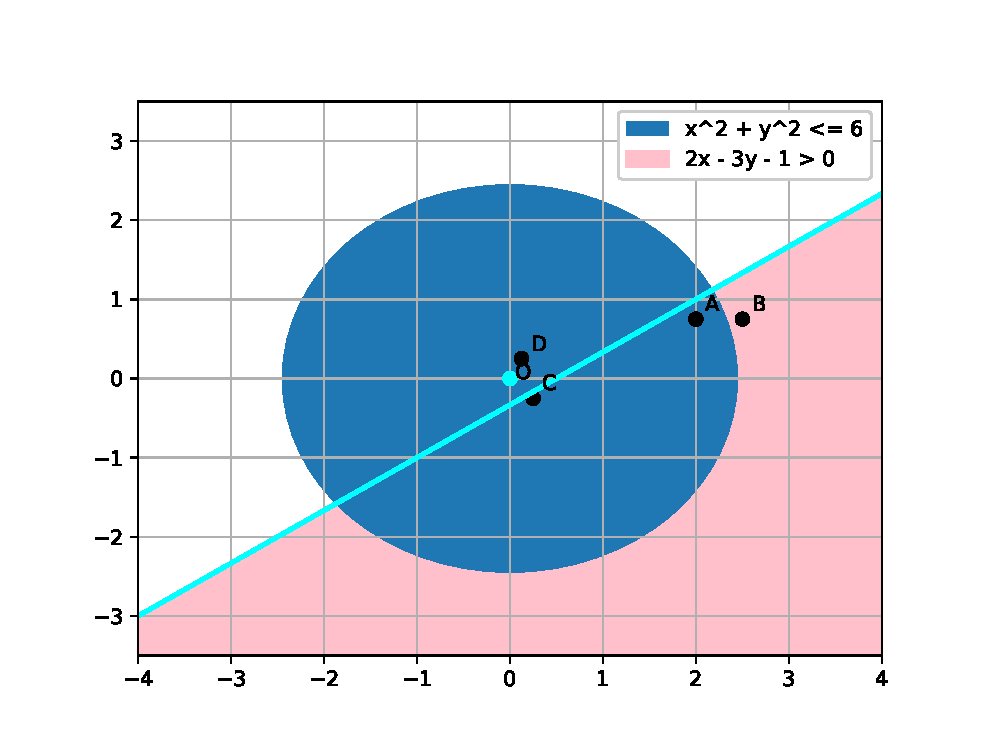
\includegraphics[scale=0.6]{/home/raghav/Desktop/EE1390-Matrix-Project/Figures/graph.eps}
\caption{Points A and C satisfy the given condition}
\label{foobar-figure}
\end{figure}

\end{frame}

\end{document}

